%% Template for MLP Coursework 2 / 6 November 2017 

%% Based on  LaTeX template for ICML 2017 - example_paper.tex at 
%%  https://2017.icml.cc/Conferences/2017/StyleAuthorInstructions

\documentclass{article}
\usepackage[T1]{fontenc}
\usepackage{amssymb,amsmath}
\usepackage{txfonts}
\usepackage{microtype}

% For figures
\usepackage{graphicx}
\usepackage{subfigure} 

% For citations
\usepackage{natbib}

% For algorithms
\usepackage{algorithm}
\usepackage{algorithmic}

% the hyperref package is used to produce hyperlinks in the
% resulting PDF.  If this breaks your system, please commend out the
% following usepackage line and replace \usepackage{mlp2017} with
% \usepackage[nohyperref]{mlp2017} below.
\usepackage{hyperref}
\usepackage{url}
\urlstyle{same}

% Packages hyperref and algorithmic misbehave sometimes.  We can fix
% this with the following command.
\newcommand{\theHalgorithm}{\arabic{algorithm}}


% Set up MLP coursework style (based on ICML style)
\usepackage{mlp2018}
\mlptitlerunning{MLP Coursework 1 (\studentNumber)}
\bibliographystyle{icml2017}


\DeclareMathOperator{\softmax}{softmax}
\DeclareMathOperator{\sigmoid}{sigmoid}
\DeclareMathOperator{\sgn}{sgn}
\DeclareMathOperator{\relu}{relu}
\DeclareMathOperator{\lrelu}{lrelu}
\DeclareMathOperator{\elu}{elu}
\DeclareMathOperator{\selu}{selu}
\DeclareMathOperator{\maxout}{maxout}

\usepackage{url}
\usepackage{graphicx} 
\usepackage{float}
\usepackage{amsmath}

%% You probably do not need to change anything above this comment

%% REPLACE this with your student number
\def\studentNumber{s1502810}

\begin{document} 

\twocolumn[
\mlptitle{MLP Coursework 2: Exploring Convolutional Networks}

\centerline{\studentNumber}

\vskip 7mm
]

\begin{abstract} 
Deep learning shines in the field of computer vision, and many problems that cannot be solved under traditional methods are being overcome. However, the high computational cost also greatly limits the use of deep learning, and its computationally intensive features are particularly prominent on platforms such as mobile devices and embedded devices.Convolutional neural networks are an important part of deep learning, especially in the field of image recognition and image processing.For most convolutional neural networks, the convolutional layer is the most time consuming part and How to efficiently perform convolutional layer calculation is the key point to improve the performance of deep learning inference\cite{JiaYangqing2014LSIR}.This report will compare the various convolution algorithms in the convolutional layer and compare their performance.After the convolutional layer, the downsampling operation is generally performed. Downsampling can reduce parameters and prevent overfitting. This report will compare the two downsampling methods of pooling and dilate convolution.

\end{abstract} 

\section{Introduction}
\label{sec:intro}

This report will discuss two parts. The first part is to explain the convolutional neural network. It mainly explains the convolutional layer and the pooling layer, and then reports the principle of implementing the two layers. Finally, it compares the advantages and disadvantages of different implementations of the convolution algorithm in the convolutional layer.In the second part, we will focus on the downsampling operation after the convolutional layer. In the classical convolutional neural network, after the general convolutional layer is processed, it will be handed over to the pooling layer for downsampling operation. The algorithm of the pooling layer is very much, classic and common are max pooling and average pooling. The role of the pooling layer is to reduce parameters and extract important features, thereby preventing network overfitting and improving the generalization ability of the network. However, relative to the downsampling of the pooling layer, the dilated convolution removes the pooled downsampling operation without reducing the network's receptive field. We will compare these two downsampling techniques in terms of accuracy, memory requirements, and fitting speed.The experiment used a variant of the NIST dataset, which we call Extended MNIST (EMNIST), which follows the same transformation paradigm as used when creating the MNIST dataset. The result is a series of data sets that make up more challenging classification tasks involving letters and numbers, and they have the same image structure and parameters as the original MNIST task, allowing for all existing classifiers and systems. 

\section{Implementing convolutional networks} 

Traditional neural networks use matrix multiplication to establish the connection between input and output, while convolutional neural networks use convolution to describe the relationship between input and output.
A convolutional neural network generally consists of five kinds of layers: input layers,convolutional layers, detector stage, pooling layers and  full connected layers. Below we will focus on the convolutional layers and the pooling layers.

\subsection{Convolutional layer}

Compared to the traditional fully connected layer, the convolution layer is faster and requires less storage space because the convolution layer has two features of sparse interactions and parameter sharing.

\textbf{sparse interactions}\\
Traditional neural networks have a relationship between each input and each output, whereas an output of a convolutional network only has a relationship with a portion of the input.This feature is achieved by making the size of the kernel much smaller than the size of the input.\cite{deeplearning2016}.

\textbf{parameter sharing}\\
In a model, the same set of parameters is used multiple times in multiple functions.\cite{deeplearning2016}.
This means that pixels in different positions of the input will operate with the same kernel, learning the same set of parameters.

Taking our experiment as an example, our input is a 28 $\times$ 28 pixel image, and we only need a 3 $\times$ 3 kernel which is used to detect some small meaningful features in the image. The output is a 26 $\times$ 26 feature map(padding = 0, stride = 1).

\begin{table}[H]
  \centering
%  \caption{compare convolutional layer with full connected layer}
    \begin{tabular}{lll}
          & convolutional layer & full connected layer \\
    parameters & 3 $\times$ 3 + 1  & 28 $\times$ 28 $\times$ 100  \\
    hidden units & 26 $\times$ 26 & 100 \\
    connections & 26 $\times$ 26 $\times$ 3 $\times$ 3 & 28 $\times$ 28 $\times$ 100 \\
    \end{tabular}%
  \label{clayertable1}
\end{table}%
The number of parameters and connections in the convolutional layer is much smaller than the fully connected layer. And if the stride is increased, the effect will be more significant.This not only reduces storage requirements, but also reduces the amount of computation.
\subsection{pooling layer}
Normally, the convolution layer will pass the result to the detector stage (for example Relu) after processing, after which the pooling layer will further adjust the data and pass to next convolution layer.pooling layer is actually a form of downsampling. There are many different forms of nonlinear pooling functions such as Max pooling and average pooling. The pooling layer will continuously reduce the size of the data space, so the number of parameters and the amount of calculation will also decrease, which also controls over-fitting to some extent.

\subsection{Implementation}

\textbf{Convolutional layer}\\
The method I use is convolve2d. With this convolution method, we only need to find the input location and kernels, and then perform the convolution calculation. Of course, we also need to consider the input channel and output channel.
\begin{figure}[H] %H为当前位置,!htb为忽略美学标准,htbp为浮动图形
	\centering %图片居中
	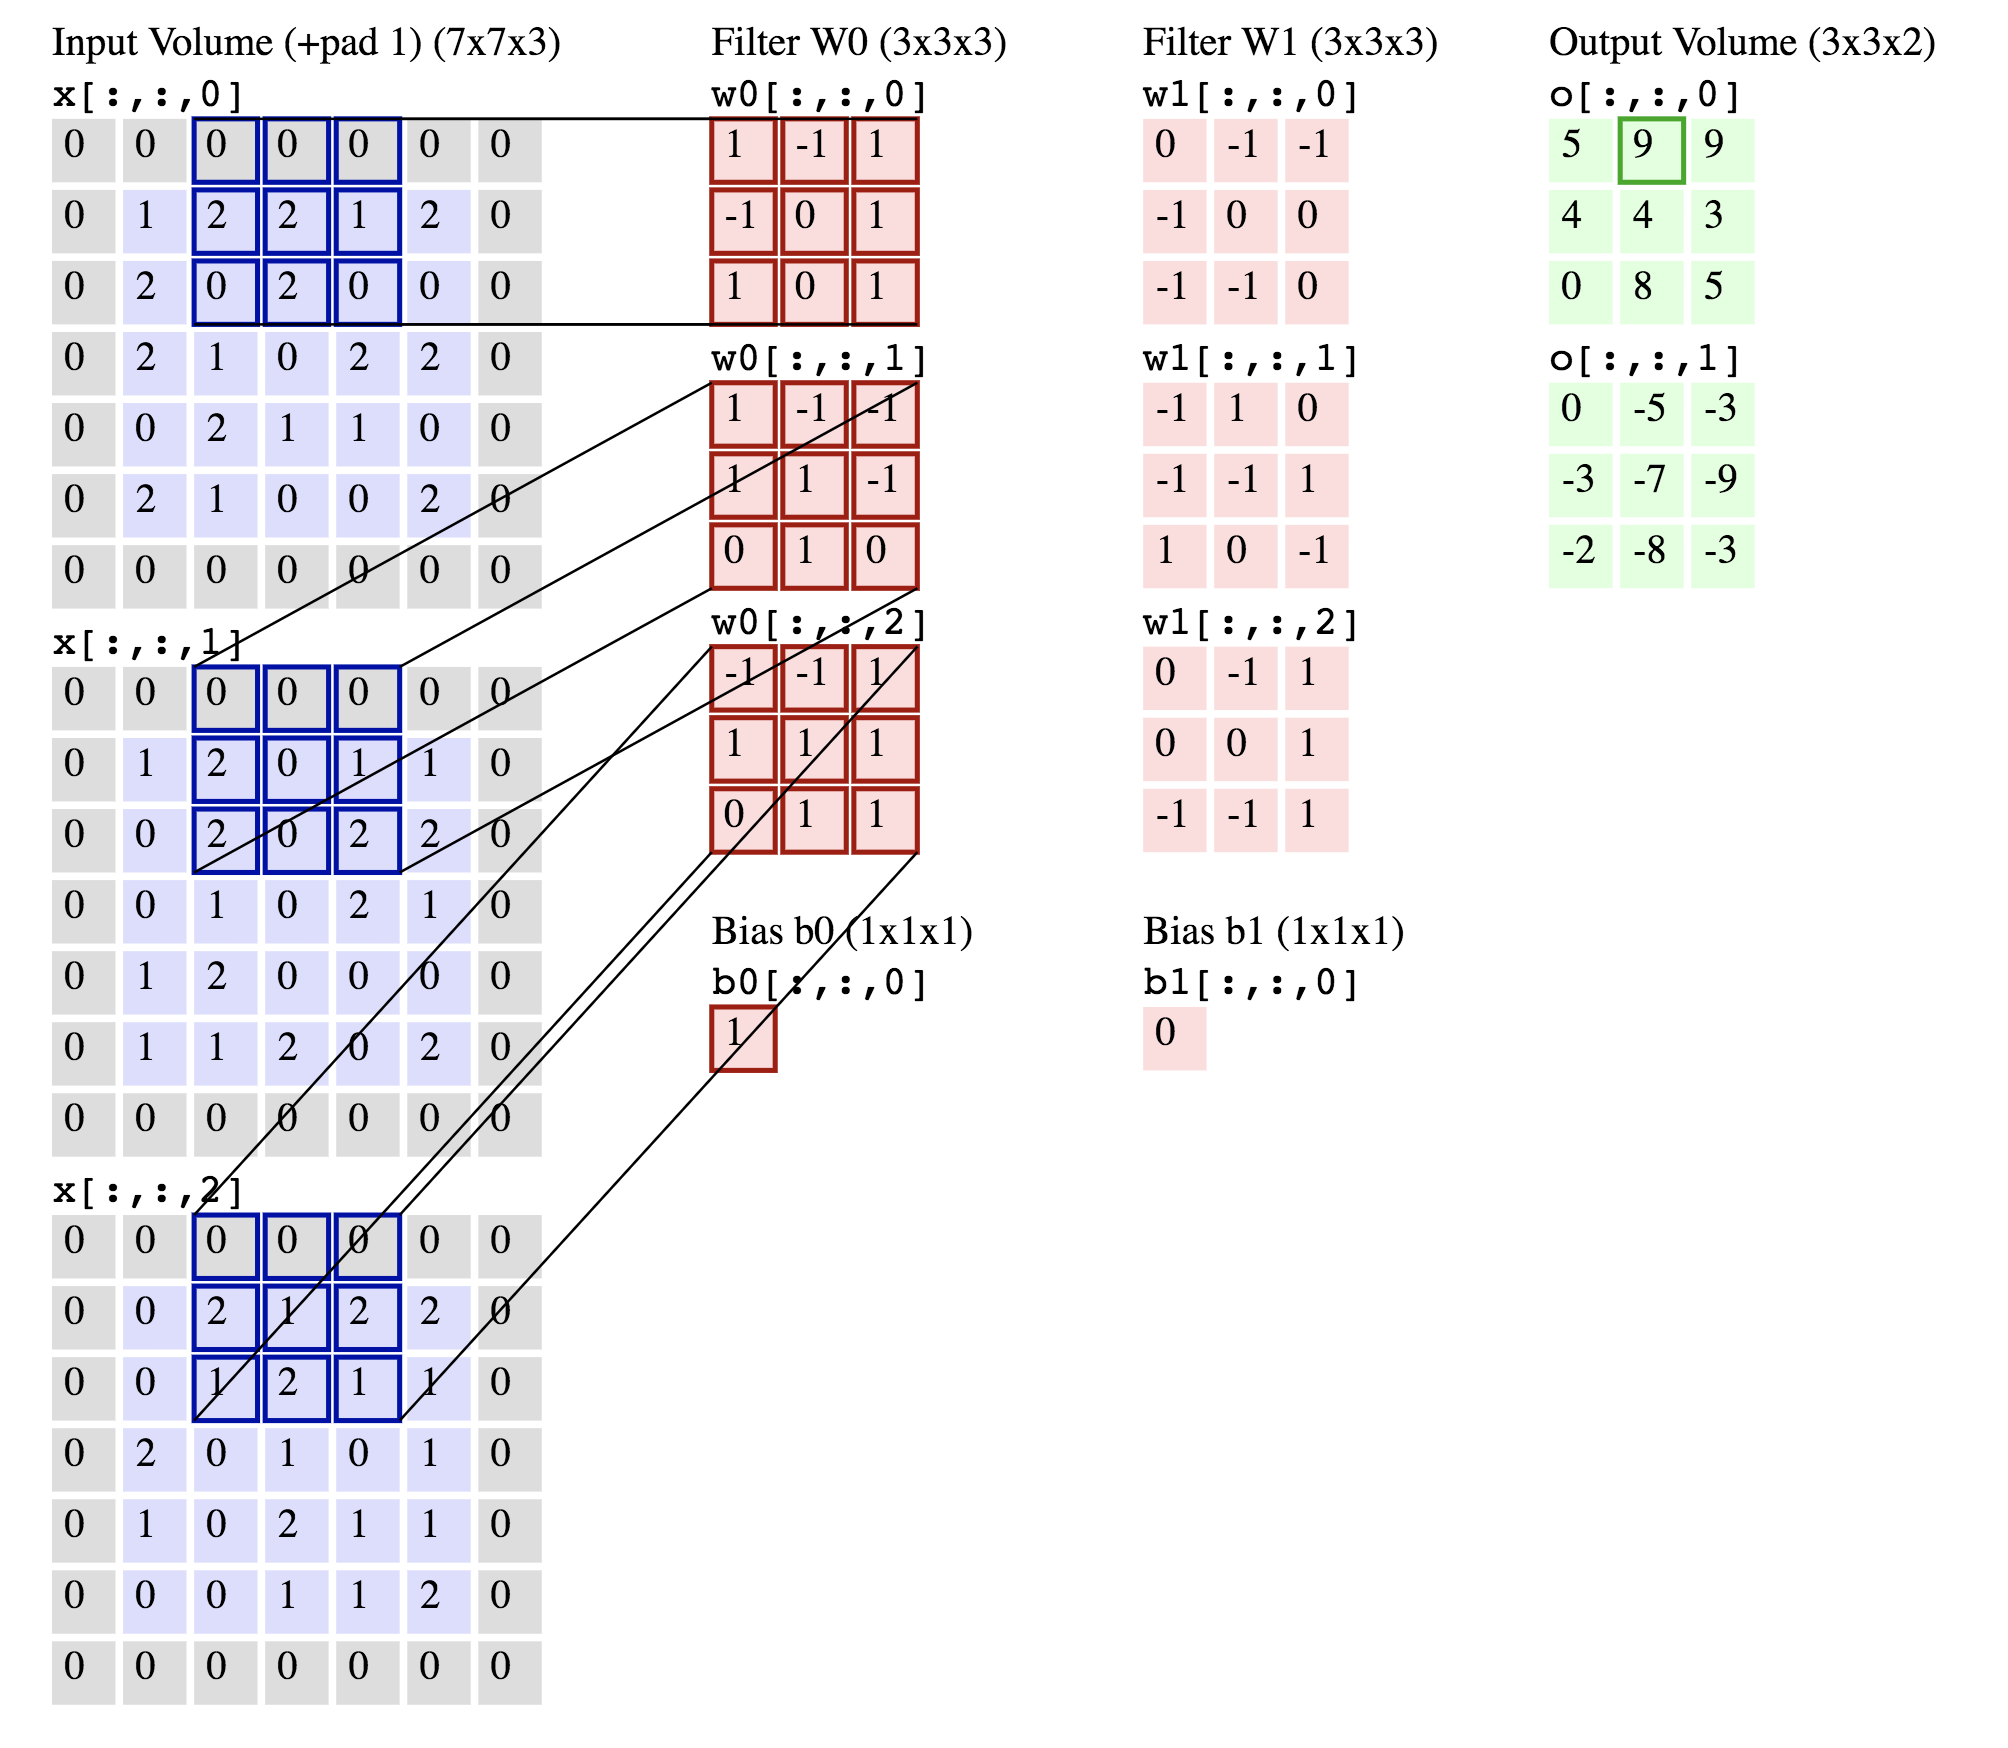
\includegraphics[width=0.45\textwidth]{./pic/part1/cnlayerImp.png} %插入图片,[]中设置图片大小,{}中是图片文件名
	\caption{convoluation layer implementation} %最终文档中希望显示的图片标题
	\label{Fig.main2} %用于文内引用的标签
	\cite{cs231n}
\end{figure}
The same is true for my implementation. I create 3 loops corresponding to batch  size, input channel and output channel, then find the input matrix of the image and the kernel matrix for convolution. After that, because there are multiple channels, I need to accumulate.For backpropagation, the implementation is similar, but it becomes the output weight and the kernel performs the convolution operation, but the kernel needs to be transposed first. For the grads wrt params function, we need input and output weights for convolution, but we need to transpose the inputs matrix first.\\

\textbf{Pooling layer}\\
The pooling algorithm I implemented is max pooling.
\begin{figure}[H] %H为当前位置,!htb为忽略美学标准,htbp为浮动图形
	\centering %图片居中
	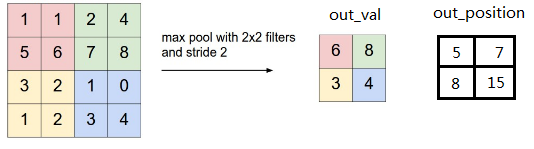
\includegraphics[width=0.5\textwidth]{./pic/part1/mpImpfprop.png} %插入图片,[]中设置图片大小,{}中是图片文件名
	\caption{maxpooling forward propagation implementation} %最终文档中希望显示的图片标题
	\label{Fig.main2} %用于文内引用的标签
\end{figure}
For the following figure, the input data X is 4*4, the sampling core size is 2, stride is 2, and no padding. The input data size is similar to the convolutional layer calculation method (input-width+2$\times$pad-pool-size)/stride+1. Forward propagation not only calculates the maximum value in the pool area, but also records the position in the input data of the maximum value. The purpose is to pass the gradient value to the position where the corresponding maximum value is in the backpropagation.
So for the backpropagation,It is known by forwardpropagation that the gradient value corresponds to the maximum position of the output of the previous layer. The specific process is as follows:
\begin{figure}[H] %H为当前位置,!htb为忽略美学标准,htbp为浮动图形
	\centering %图片居中
	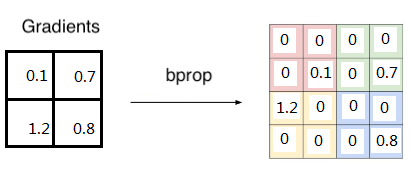
\includegraphics[width=0.5\textwidth]{./pic/part1/mpImpBprop.png} %插入图片,[]中设置图片大小,{}中是图片文件名
	\caption{maxpooling backpropagation implementation} %最终文档中希望显示的图片标题
	\label{Fig.main2} %用于文内引用的标签
\end{figure}
\subsection{Different approaches to implementing convolutional layers}
Here we will discuss three algorithms which are used for convolutional layer calculations, namely, correlate2d, im2col and Fast Fourier Transforms.
Correlate2d is a traditional convolution algorithm, although there is no advantage in speed compared to the other two, but in storage, no additional storage requirements are required.

Im2col is the multiplication of the convolution calculation into two matrices: 1. Convert the image into a matrix using im2col; 2. Convert the convolution kernel into a matrix using im2col; 3. Multiply the matrix from the first two steps.If stride < kernel size, then a large number of repeating pixels will be included in the matrix after the conversion, which is a big drain for memory. This is an obvious disadvantage of im2col for convolution operations, but this shortcoming is negligible compared to the speed gain of multiplying large matrices.

The process using the Fourier algorithm is such that the convolution in the time domain is equal to the product in the frequency domain, so after transforming our image (input) and kernel into the frequency domain, we multiply them directly, and then Transform back to the time domain. This completes the convolution operation.Because the size of a general convolution kernel is smaller than the image, we need to extend our kernel to match the size of the image.So you need to use the loop fill method to expand the convolution kernel so that the last two signals can be the same size when multiplied.The advantage of convolution calculations in the above manner is obvious - greatly reducing the amount of computation for direct convolution operations in the time domain.The disadvantages are also very obvious, because in a general convolutional neural network, the kernel is much smaller than the input, so additional memory space is needed when converting the kernel. Fourier's multiplication calculation is more complicated.

In summary, although im2col requires more memory space, it has an advantage in speed. Traditional convolution operations do not require extra memory space, but there is no advantage in speed. The memory space required by the Fourier algorithm and the efficiency of the algorithm are closely related to the size of kernal. When the core is large, the memory requirement is small, and the algorithm is efficient, and vice versa.

\section{Context in convolutional networks}

The pooling layer is a very important layer in the neural network, which not only can further extract features, but also reduce the dimensions of the next input. The first experiment in this study was to study the different performance of the two methods of average pooling and max pooling in convolutional neural networks. Here we need to understand the pooling layer more deeply.

\subsection{pooling layer}

\textbf{invariance}\\
When the input of this layer undergoes a small amount of translation and rotation, the output obtained will not change after being processed by the pooling function\cite{deeplearning2016}.This means that we are more concerned with the existence of a feature rather than the location of the specific feature.This is a very useful feature.For example,For the mnist dataset, because of the handwriting reason, the different number "1" may be in the left-hand side, the right-hand position, or a small amount of rotation relative to the standard one. But after the pooling function, the "1" they showed was consistent.

\textbf{Reduce the input of next layer}\\
Each area entered will perform pooling functions (such as max pooling, average pooling, etc.) to further extract features, reduce input dimensions, and output smaller dimensions.
\begin{figure}[H] %H为当前位置,!htb为忽略美学标准,htbp为浮动图形
	\centering %图片居中
	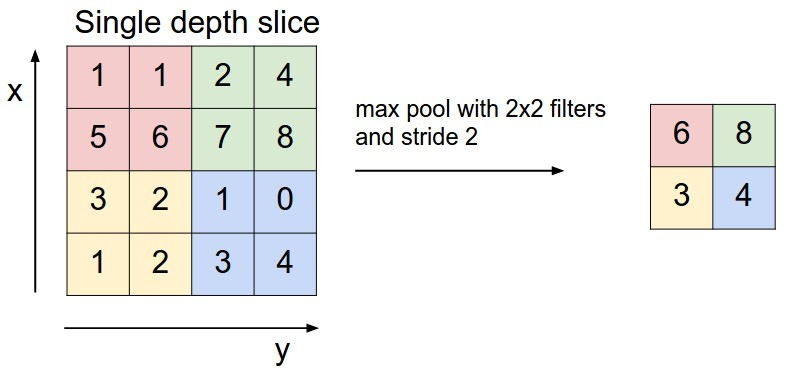
\includegraphics[width=0.4\textwidth]{./pic/part1/maxpool.jpeg} %插入图片,[]中设置图片大小,{}中是图片文件名
	\caption{Maxpooling} %最终文档中希望显示的图片标题
	\label{Fig.main2} %用于文内引用的标签
	\cite{cs231n}
\end{figure}
This image shows that After max pooling, the input has been reduced from 4 $\times$ 4 to 2 $\times$ 2.
It is precisely because the pooling function further extracts features that there are two effective functions. One is to enhance the fitting. Because the features are more obvious, the model is easier to learn the main features, and the generalization ability is strengthened. The other is to prevent over-fitting, because during the extraction process, only the main features are retained, and some relatively weak features are lost, which can prevent the model from over-fitting.

\subsection{Dilated convolution}

The second experiment I will compare two kinds of method of downsampling,average pooling and dilated convolution.

When the image is compressed in digital image processing, the matrix of N$\times$N becomes (N/2)$\times$(N/2). This step is to downsample the original image.In convolutional neural networks, average pooling is a downsampling method that compresses images and reduces input matrices.

Dilated Convolution can be one of another methods of downsample.Compared with the ordinary convolution, the expansion convolution has a dilation rate parameter in addition to the size of the convolution kernel, which is mainly used to indicate the size of the expansion. The same thing about the expansion convolution and the ordinary convolution is that the size of the convolution kernel is the same. In the neural network, the number of parameters is the same, the difference is that the expansion convolution has a larger receptive field\cite{DBLP:journals/corr/YuK15}.
\begin{figure}[H] %H为当前位置,!htb为忽略美学标准,htbp为浮动图形
	\centering %图片居中
	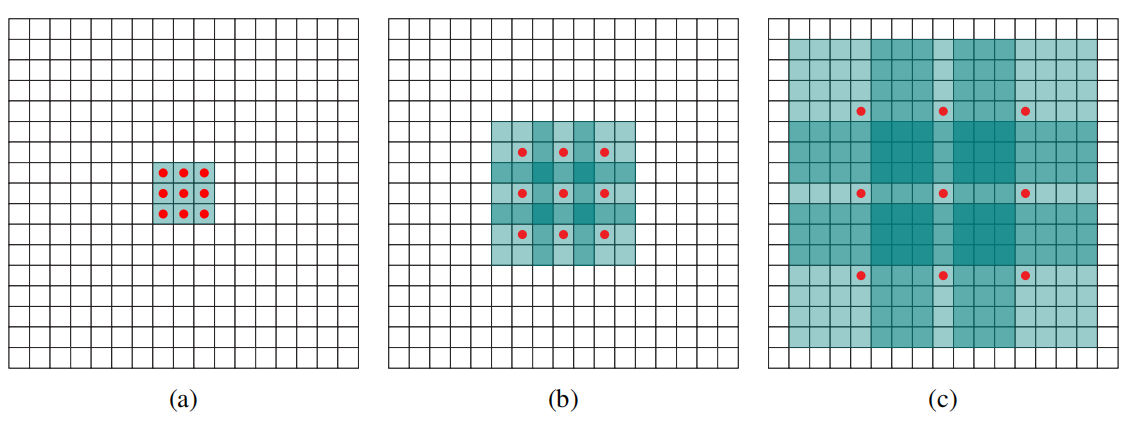
\includegraphics[width=0.44\textwidth]{./pic/part2/kongdongjuanji.png} %插入图片,[]中设置图片大小,{}中是图片文件名
	\caption{receptive field in different layer} %最终文档中希望显示的图片标题
	\label{Fig.main2} %用于文内引用的标签
	\cite{DBLP:journals/corr/YuK15}
\end{figure}

\begin{equation}
r=2^{\frac{rate}2\;+\;2}\;-\;1
\end{equation}
Use this formula to calculate the receptive field of Dilated Convolution. Rate in the equation means the dilation rate which we will increase  on each layer.As can be seen from the figure\ref{Fig.main2}, the receptive field in Fig. a is 3$\times$3=9, the receptive field in Fig. b is 7$\times$7=49, and the receptive field in Fig. c is 15$\times$15=225.The number of parameters of the convolution kernel remains unchanged, and the size of the receptive field increases exponentially with the increase of the "dilation rate" parameter.


\section{Experiments}

\subsection{Experiment  Environment}

To reduce external errors, we use Pytorch to build our convolutional neural network. This experiment also uses K80 GPU acceleration, and the running platform is built on Google Cloud.

\subsection{Convolutional neural network structure}
In this experiment we used We use a structure similar to the LeNet neural network.\cite{LecunY.1998Glat}.Because this structure has a very good effect on handwritten digit recognition. It is also relatively simple and can reduce the impact of complex network structures on experimental results.The structure of the neural network is as follows:
\begin{figure}[H] %H为当前位置,!htb为忽略美学标准,htbp为浮动图形
	\centering %图片居中
	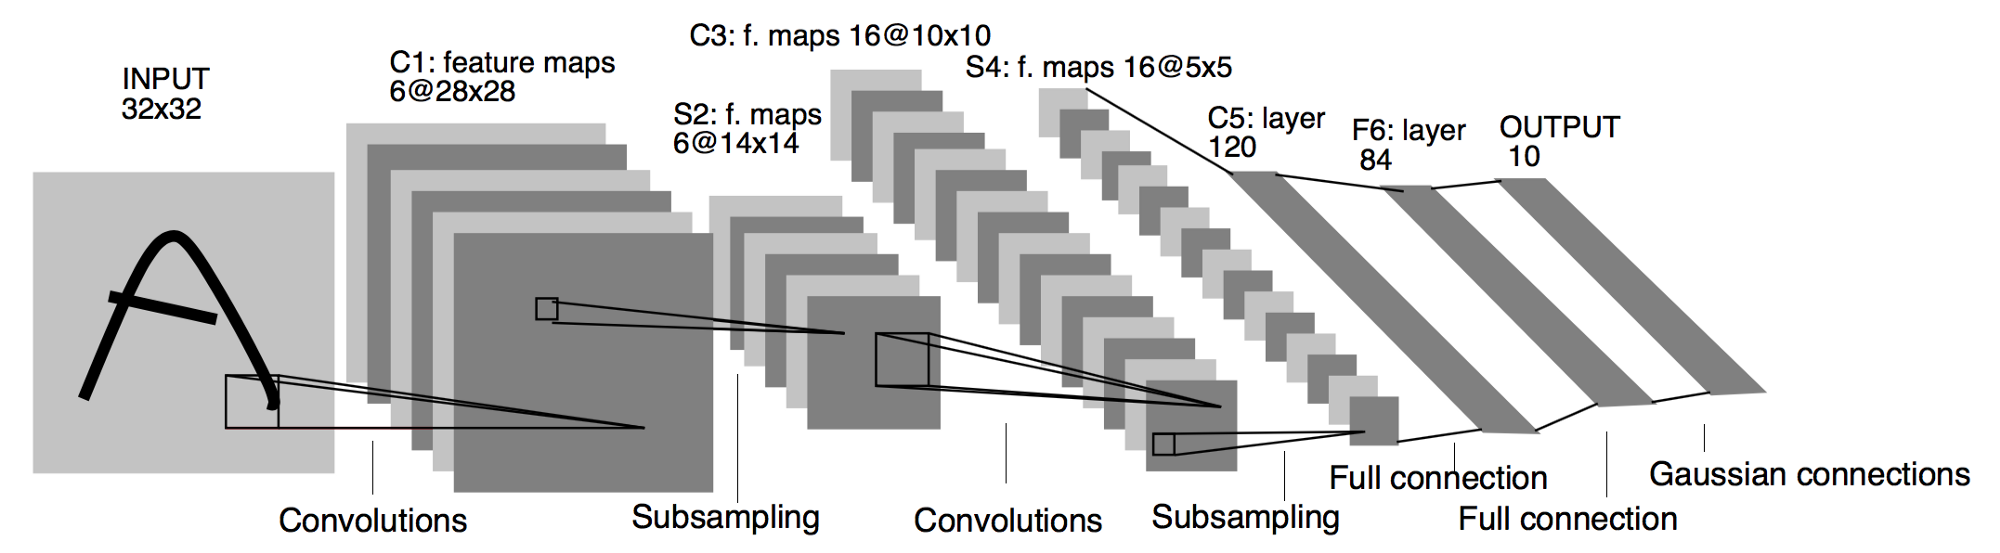
\includegraphics[width=0.5\textwidth]{./pic/part2/lenet.png} %插入图片,[]中设置图片大小,{}中是图片文件名
	\caption{LeNet} %最终文档中希望显示的图片标题
	\label{Fig.main2} %用于文内引用的标签
	\cite{LecunY.1998Glat}
\end{figure}

In this report we will change two hyperparameters: convolution layer and filters

\subsection{Compare max pooling and average pooling}
\begin{table}[htbp]
  \centering
  \caption{Constant hyperparameter}
    \begin{tabular}{lr}
    \textbf{Constant hyperparameter} & \ \textbf{value} \\
    batch\_size & 100 \\
    number of epoch & 100 \\
    number of imageChannel & 1 \\
    weight decay for Adam & 1.00E-05 \\
    \end{tabular}%
  \label{tab:addlabel}%
\end{table}%

\begin{table}[htbp]
  \centering
  \caption{Changed hyperparameter}
    \begin{tabular}{ll}
    \textbf{Changed hyperparameter} & \textbf{value range} \\
    number of layers & [1,2,3,4] \\
    filters & [2,3] \\
    \end{tabular}%
  \label{tab:addlabel}%
\end{table}%
In order to compare the accuracy, the fiiting time and computing time of max pooling and average pooling, the number of convolution layers I chose from layer 1 to layer 4, because the number of convolution layers in LeNet was two layers, the effect is quite good. I believe that the 4-layer convolution layer is sufficient for this data set. Moreover, the input itself is not large (784 pixel data). After multiple pooling layer dimensional reduction, the final dimension will become very small.
\begin{figure}[H] %H为当前位置,!htb为忽略美学标准,htbp为浮动图形
	\centering %图片居中
	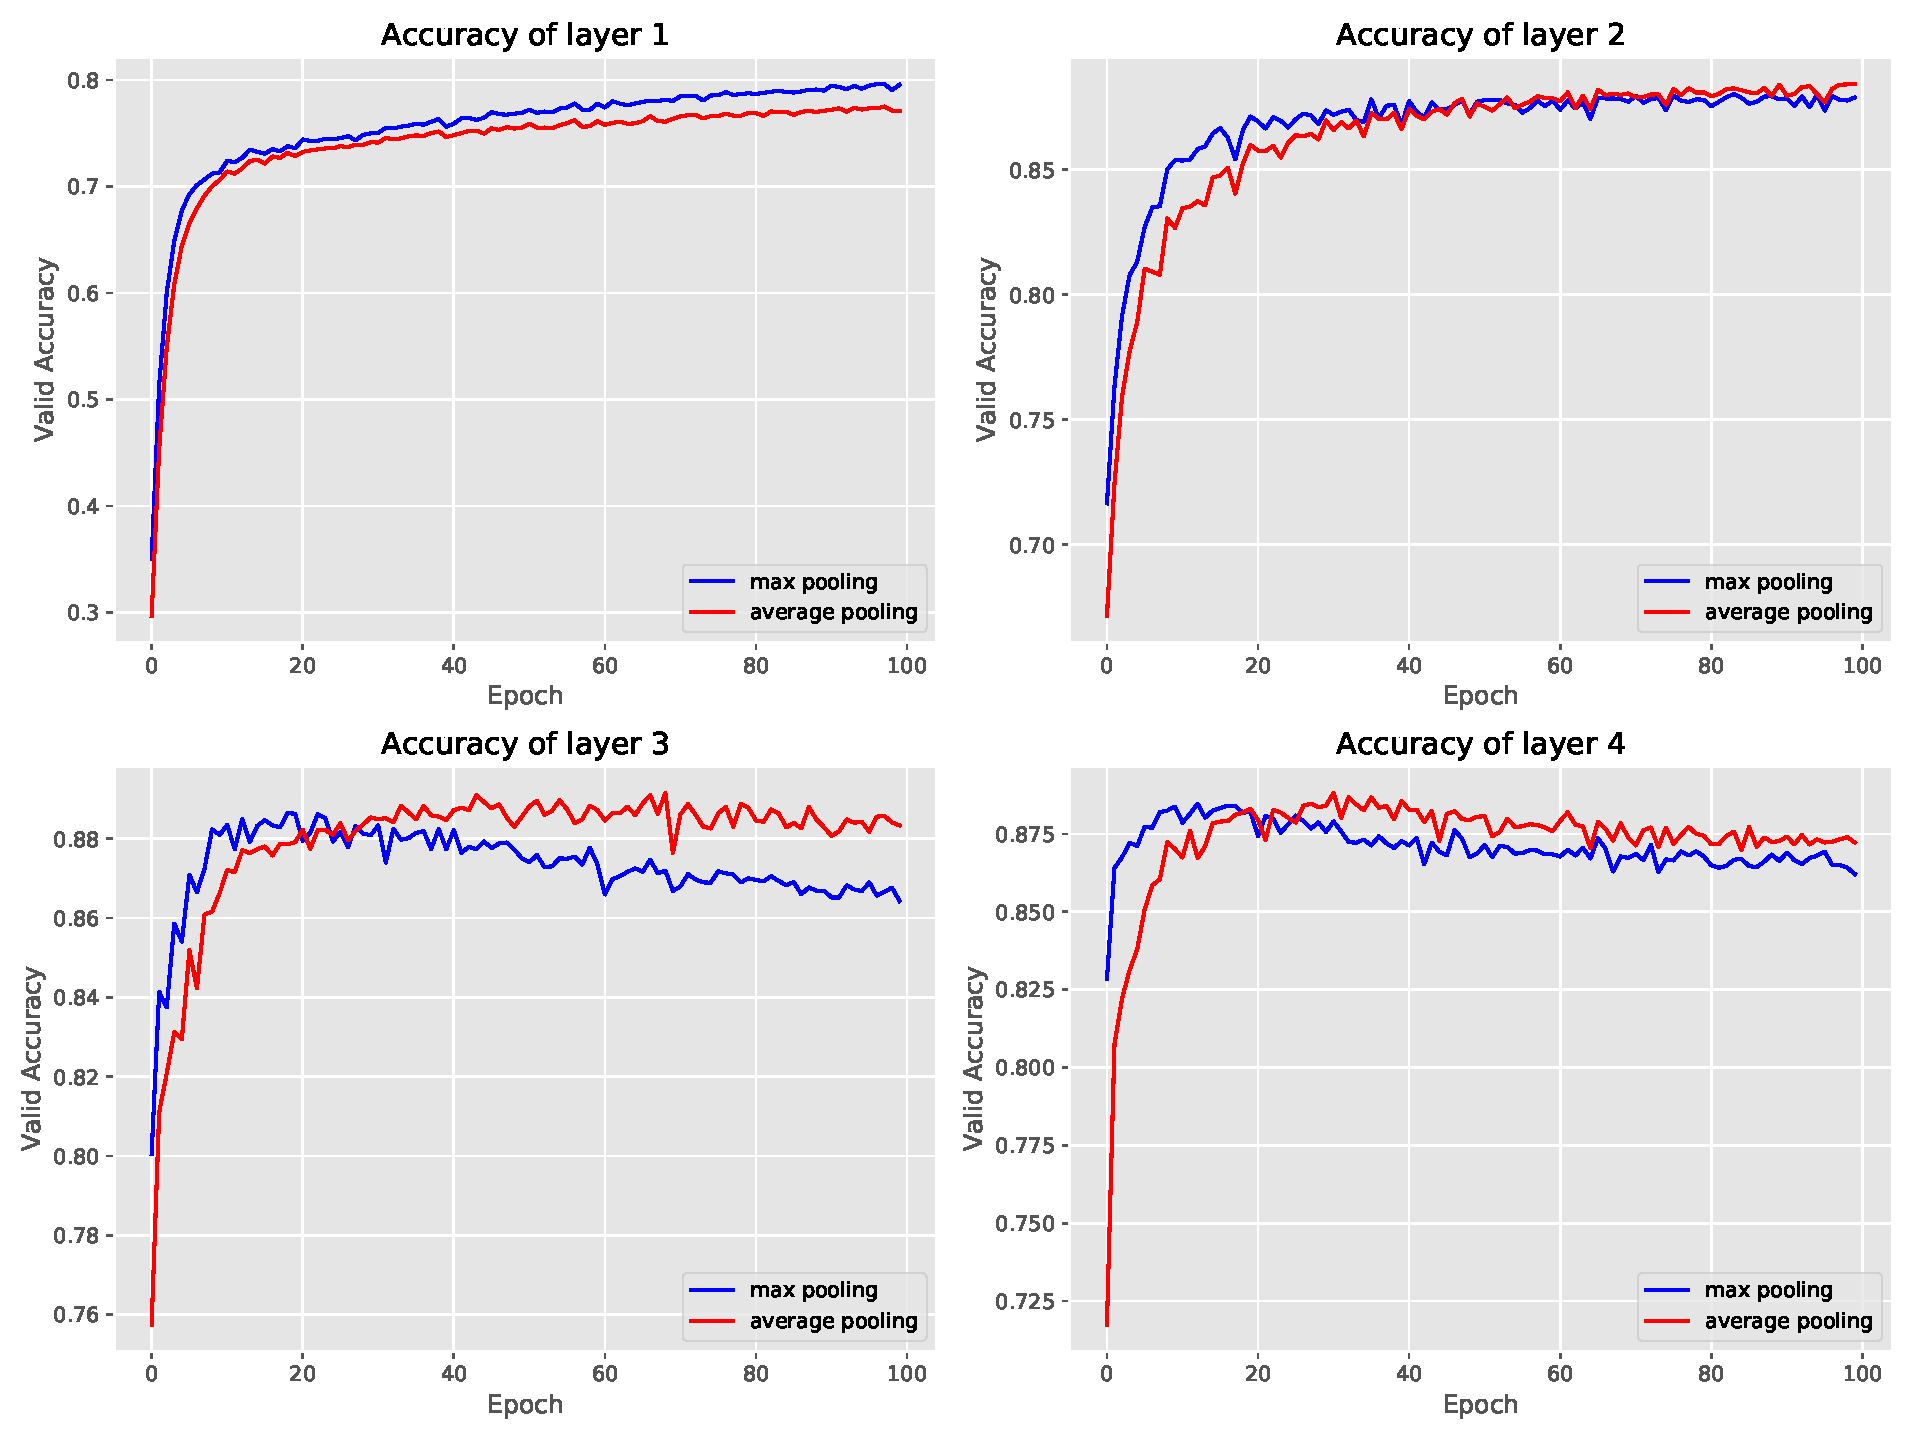
\includegraphics[width=0.44\textwidth]{./pic/part2/max_average_layer_acc.pdf} %插入图片,[]中设置图片大小,{}中是图片文件名
	\caption{Accuracy of different layers with filter = 64} %最终文档中希望显示的图片标题
	\label{Fig.main2} %用于文内引用的标签
\end{figure}
\begin{figure}[H] %H为当前位置,!htb为忽略美学标准,htbp为浮动图形
	\centering %图片居中
	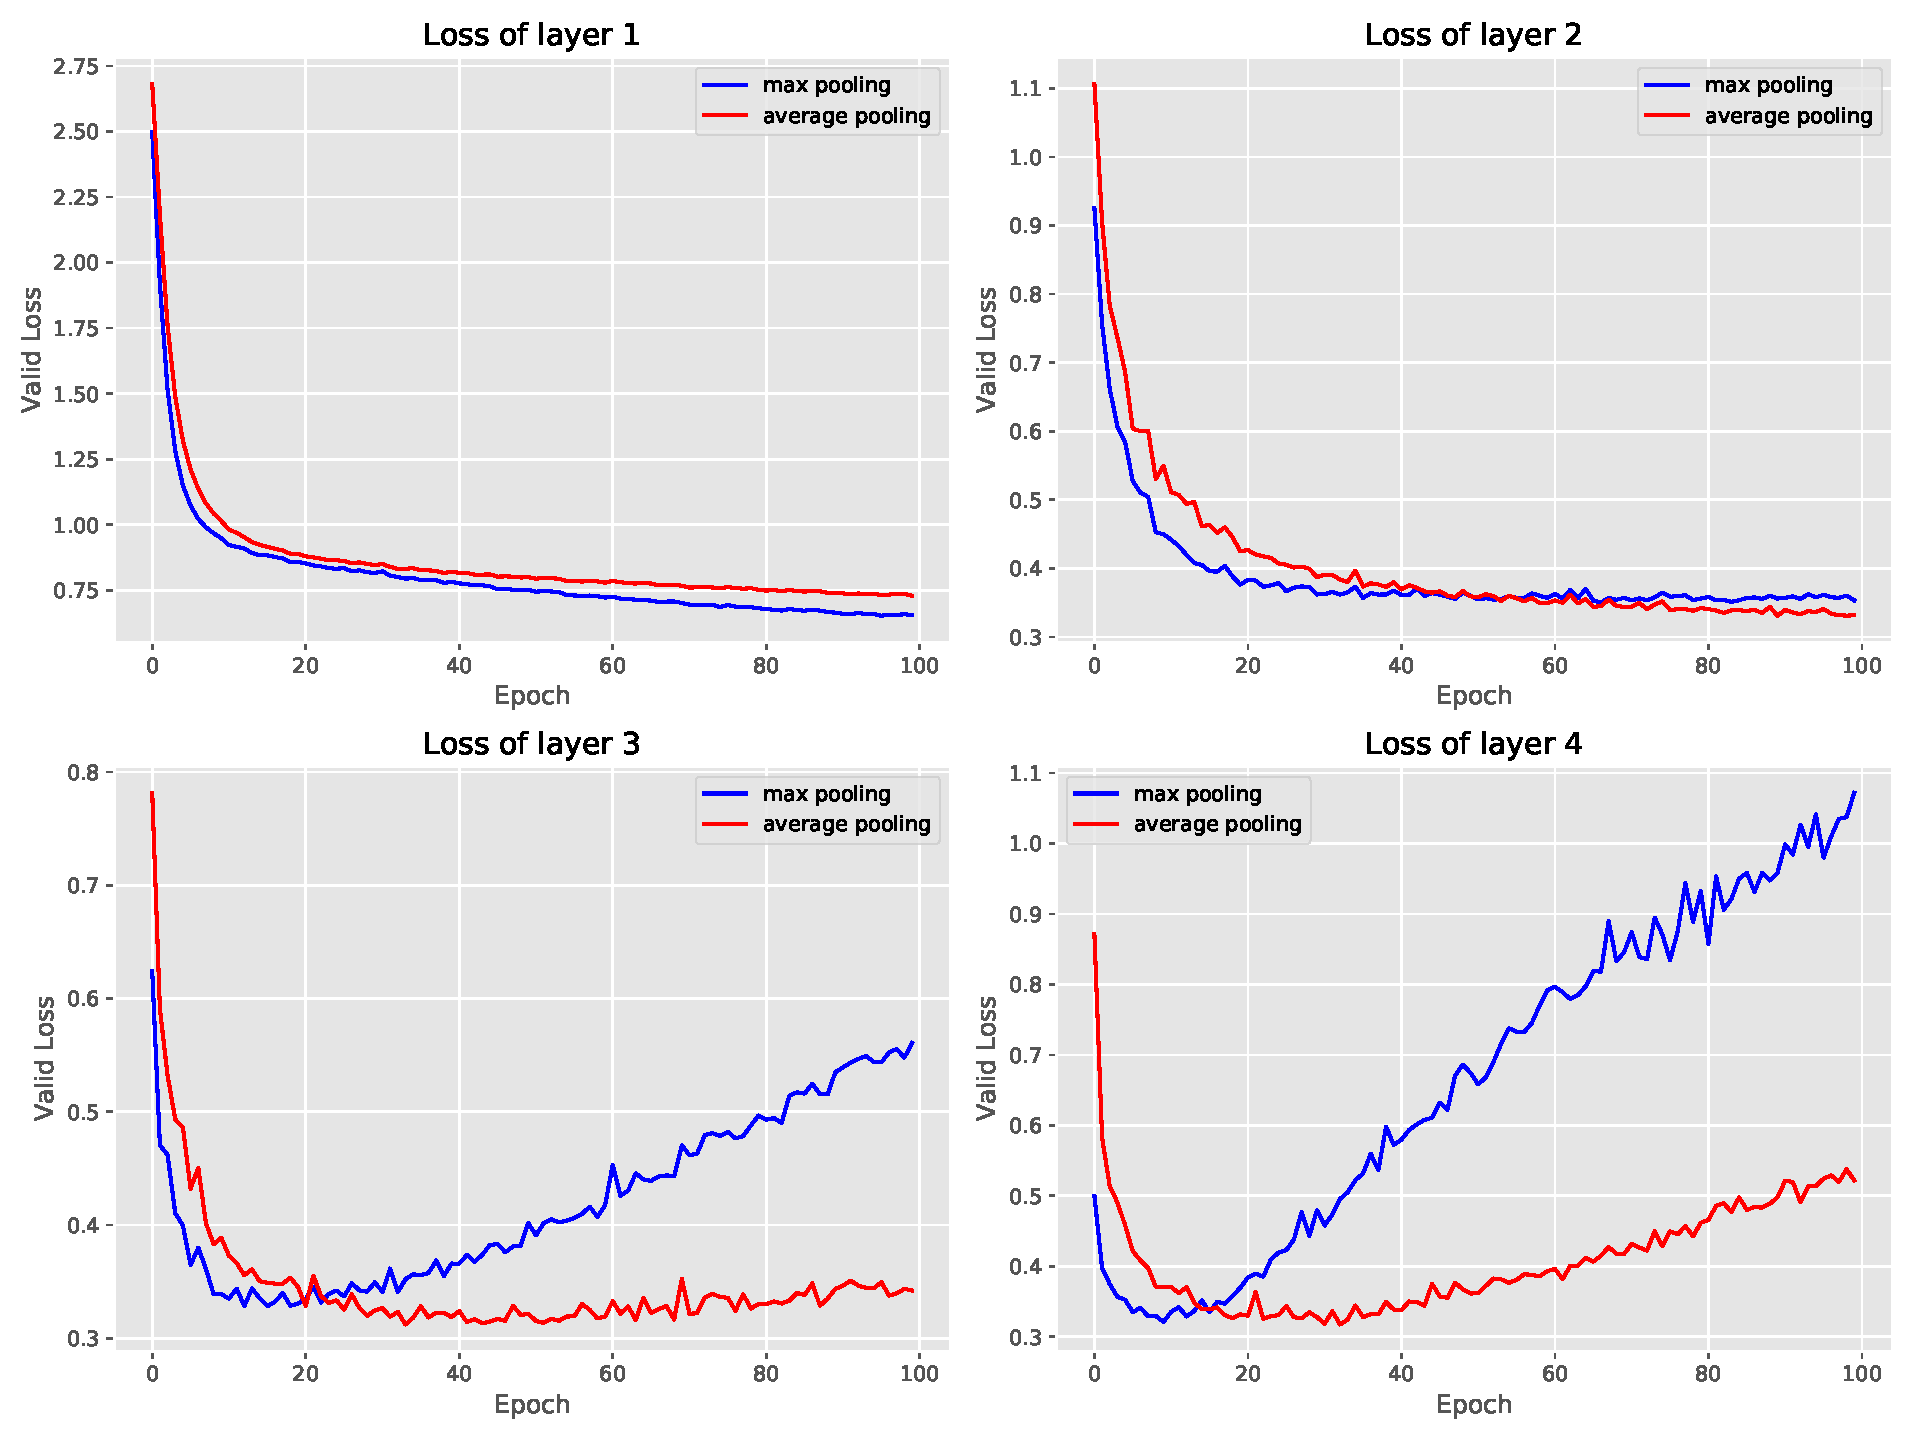
\includegraphics[width=0.44\textwidth]{./pic/part2/max_average_layer_loss.pdf} %插入图片,[]中设置图片大小,{}中是图片文件名
	\caption{Loss of different layers with filter = 64} %最终文档中希望显示的图片标题
	\label{Fig.main2} %用于文内引用的标签
\end{figure}
From the graph of accuracy, we can see that when the layer is 1, the accuracy of max pooling will be higher than that of average pooling, but the overall accuracy of layer is not high, which is an under-fitting model..When the layer is 2, the model learning is good. At this time, you can see that the accuracy of max pooling and average pooling is not much different. When layer=3, max pooling has an overfitting situation, so the accuracy of average pooling is much better than max pooling. When the layer is 4, both models have over-fitting, so the accuracy is not high.Because there are different degrees of overfitting in layer=3 and layer=4, we reduce the filter to 32 and revisit the max pooling and average pooling cases.


\begin{figure}[H] %H为当前位置,!htb为忽略美学标准,htbp为浮动图形
	\centering %图片居中
	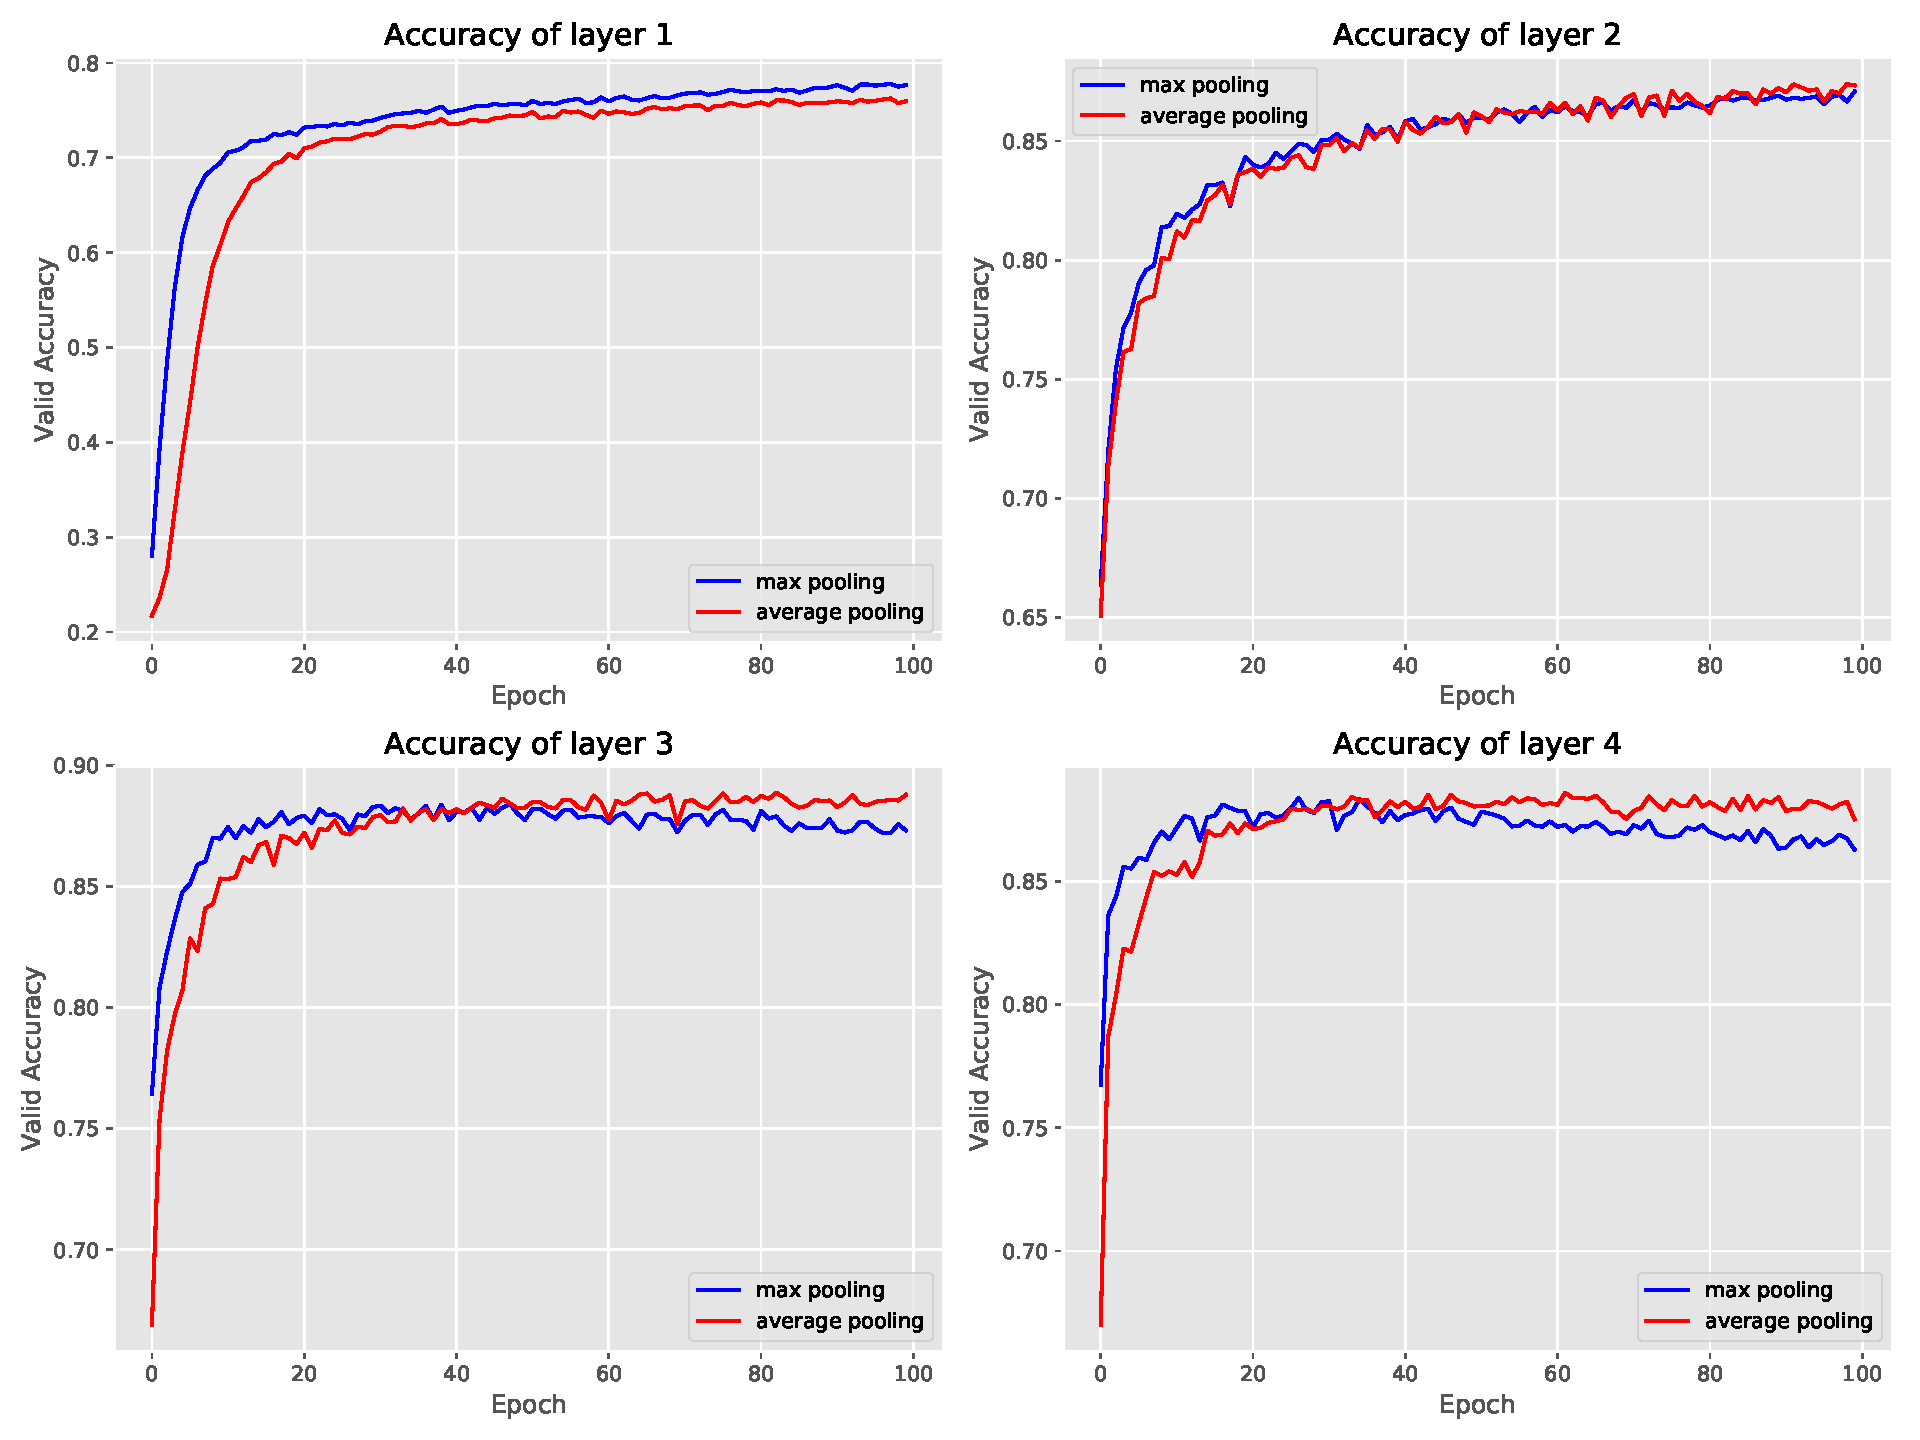
\includegraphics[width=0.44\textwidth]{./pic/part2/filter32_max_average_layer_acc.pdf} %插入图片,[]中设置图片大小,{}中是图片文件名
	\caption{Accuracy of different layers with filter = 32} %最终文档中希望显示的图片标题
	\label{Fig.main2} %用于文内引用的标签
\end{figure}

\begin{figure}[H] %H为当前位置,!htb为忽略美学标准,htbp为浮动图形
	\centering %图片居中
	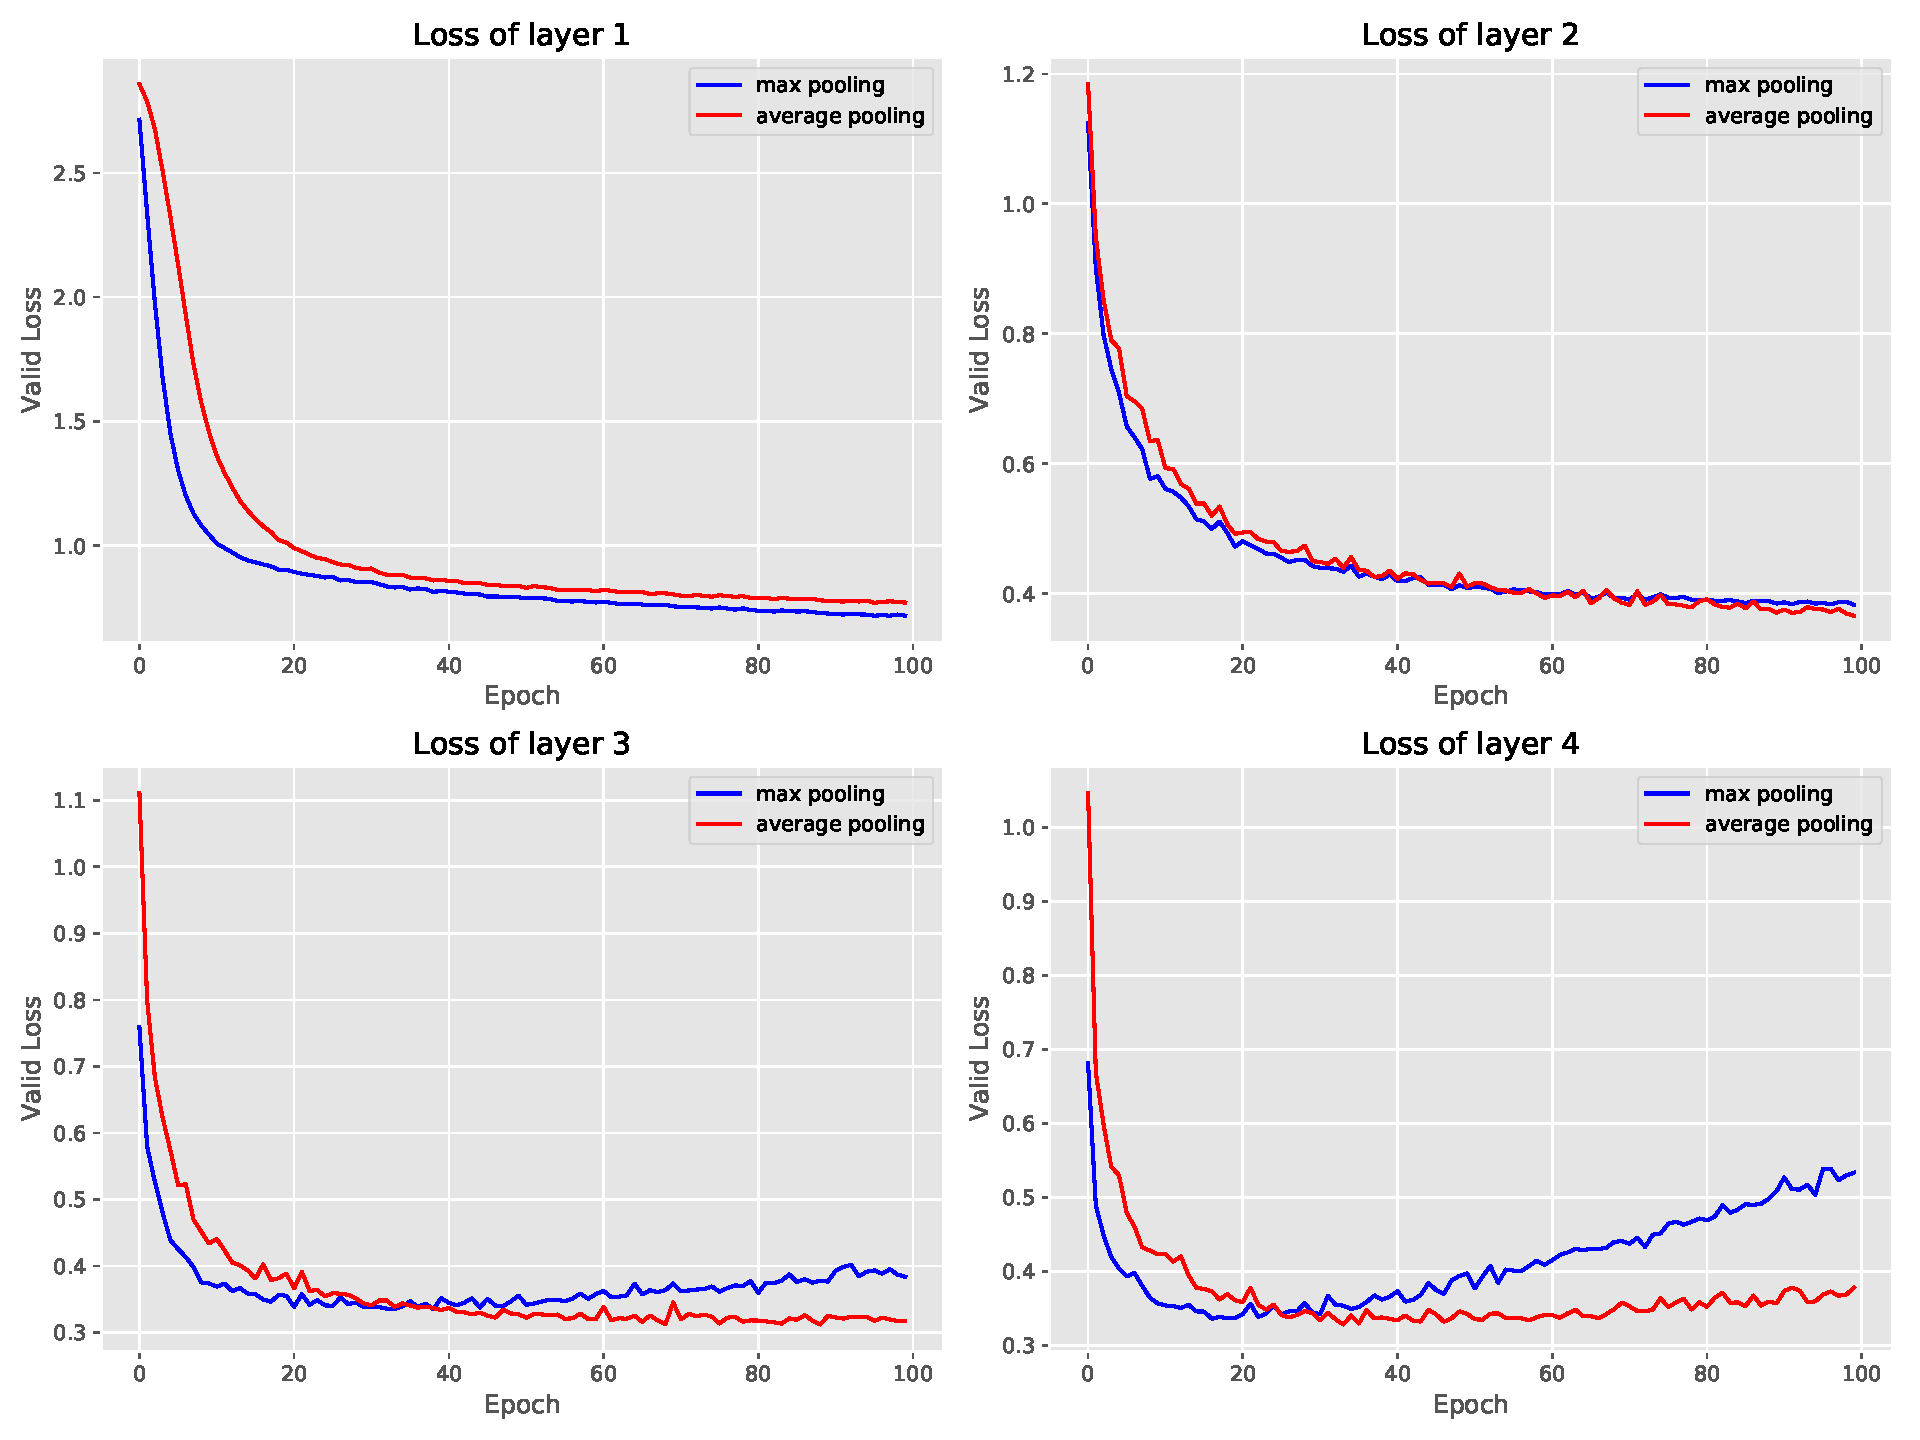
\includegraphics[width=0.44\textwidth]{./pic/part2/filter32_max_average_layer_loss.pdf} %插入图片,[]中设置图片大小,{}中是图片文件名
	\caption{Loss of different layers with filter = 32} %最终文档中希望显示的图片标题
	\label{Fig.main2} %用于文内引用的标签
\end{figure}

\textbf{Accuracy}

% Table generated by Excel2LaTeX from sheet 'Sheet1'
\begin{table}[htbp]
  \centering
  \caption{Accuracy of Different layers for Test set}
    \begin{tabular}{lrr}
          & \multicolumn{1}{l}{max pooling} & \multicolumn{1}{l}{average pooling} \\
    layer1 & 0.77158228 & 0.752341772 \\
    layer2 & 0.86245665 & 0.86398734 \\
    layer3 & 0.87493671 & 0.88012658 \\
    layer4 & 0.87360759 & 0.87689873 \\
    \end{tabular}%
  \label{tab:addlabel}%
\end{table}%


It can be seen from the figure that when both models are under-learning, the accuracy of max pooling will be higher than that of average pooling. If the model is fitted properly, the accuracy of the two will not be the same.

\textbf{Fitting speed}
In the case of under-fitting, max pooling will be better than average, because max pooling's ability to extract features is more powerful. In the case of the same number of filters, max pooling will have more learning ability than average. The advantage is that the fitting speed is faster, but the disadvantage is that too many features will be learned, resulting in faster over-fitting.In fact, it is not difficult to explain why the max pooling fitting speed will be faster. Because in the calculation method, max pooling will select the maximum value in the receptive field, and average pooling is to calculate the average value of the receptive field. The max pooling approach is more radical and maximizes the extraction of key features.

\textbf{Runtime}

% Table generated by Excel2LaTeX from sheet 'Sheet1'
\begin{table}[H]
  \centering
  \caption{Calculation time per epoch (seconds)}
    \begin{tabular}{lrr}
          & \multicolumn{1}{l}{max pooling} & \multicolumn{1}{l}{average pooling} \\
    layer=1 & 12.88 & 13.2 \\
    layer=2 & 19.34 & 19.81 \\
    layer=3 & 21.6  & 22.26 \\
    layer=4 & 23.4  & 23.85 \\
    \end{tabular}%
  \label{tab:addlabel}%
\end{table}%

We noticed that the two poolings have little difference in computing time, and the average pooling takes less than a second, because the calculation of the average is one more time than the calculation of the maximum value.

In conlusion,Max pooling has the ability to extract features more quickly and fit faster. The accuracy of the average pooling will be slightly higher than the max pooling. Calculating speed, average pool takes more time than max pooling.

\subsection{Compare average pooling  and dilation}



\begin{figure}[H] %H为当前位置,!htb为忽略美学标准,htbp为浮动图形
	\centering %图片居中
	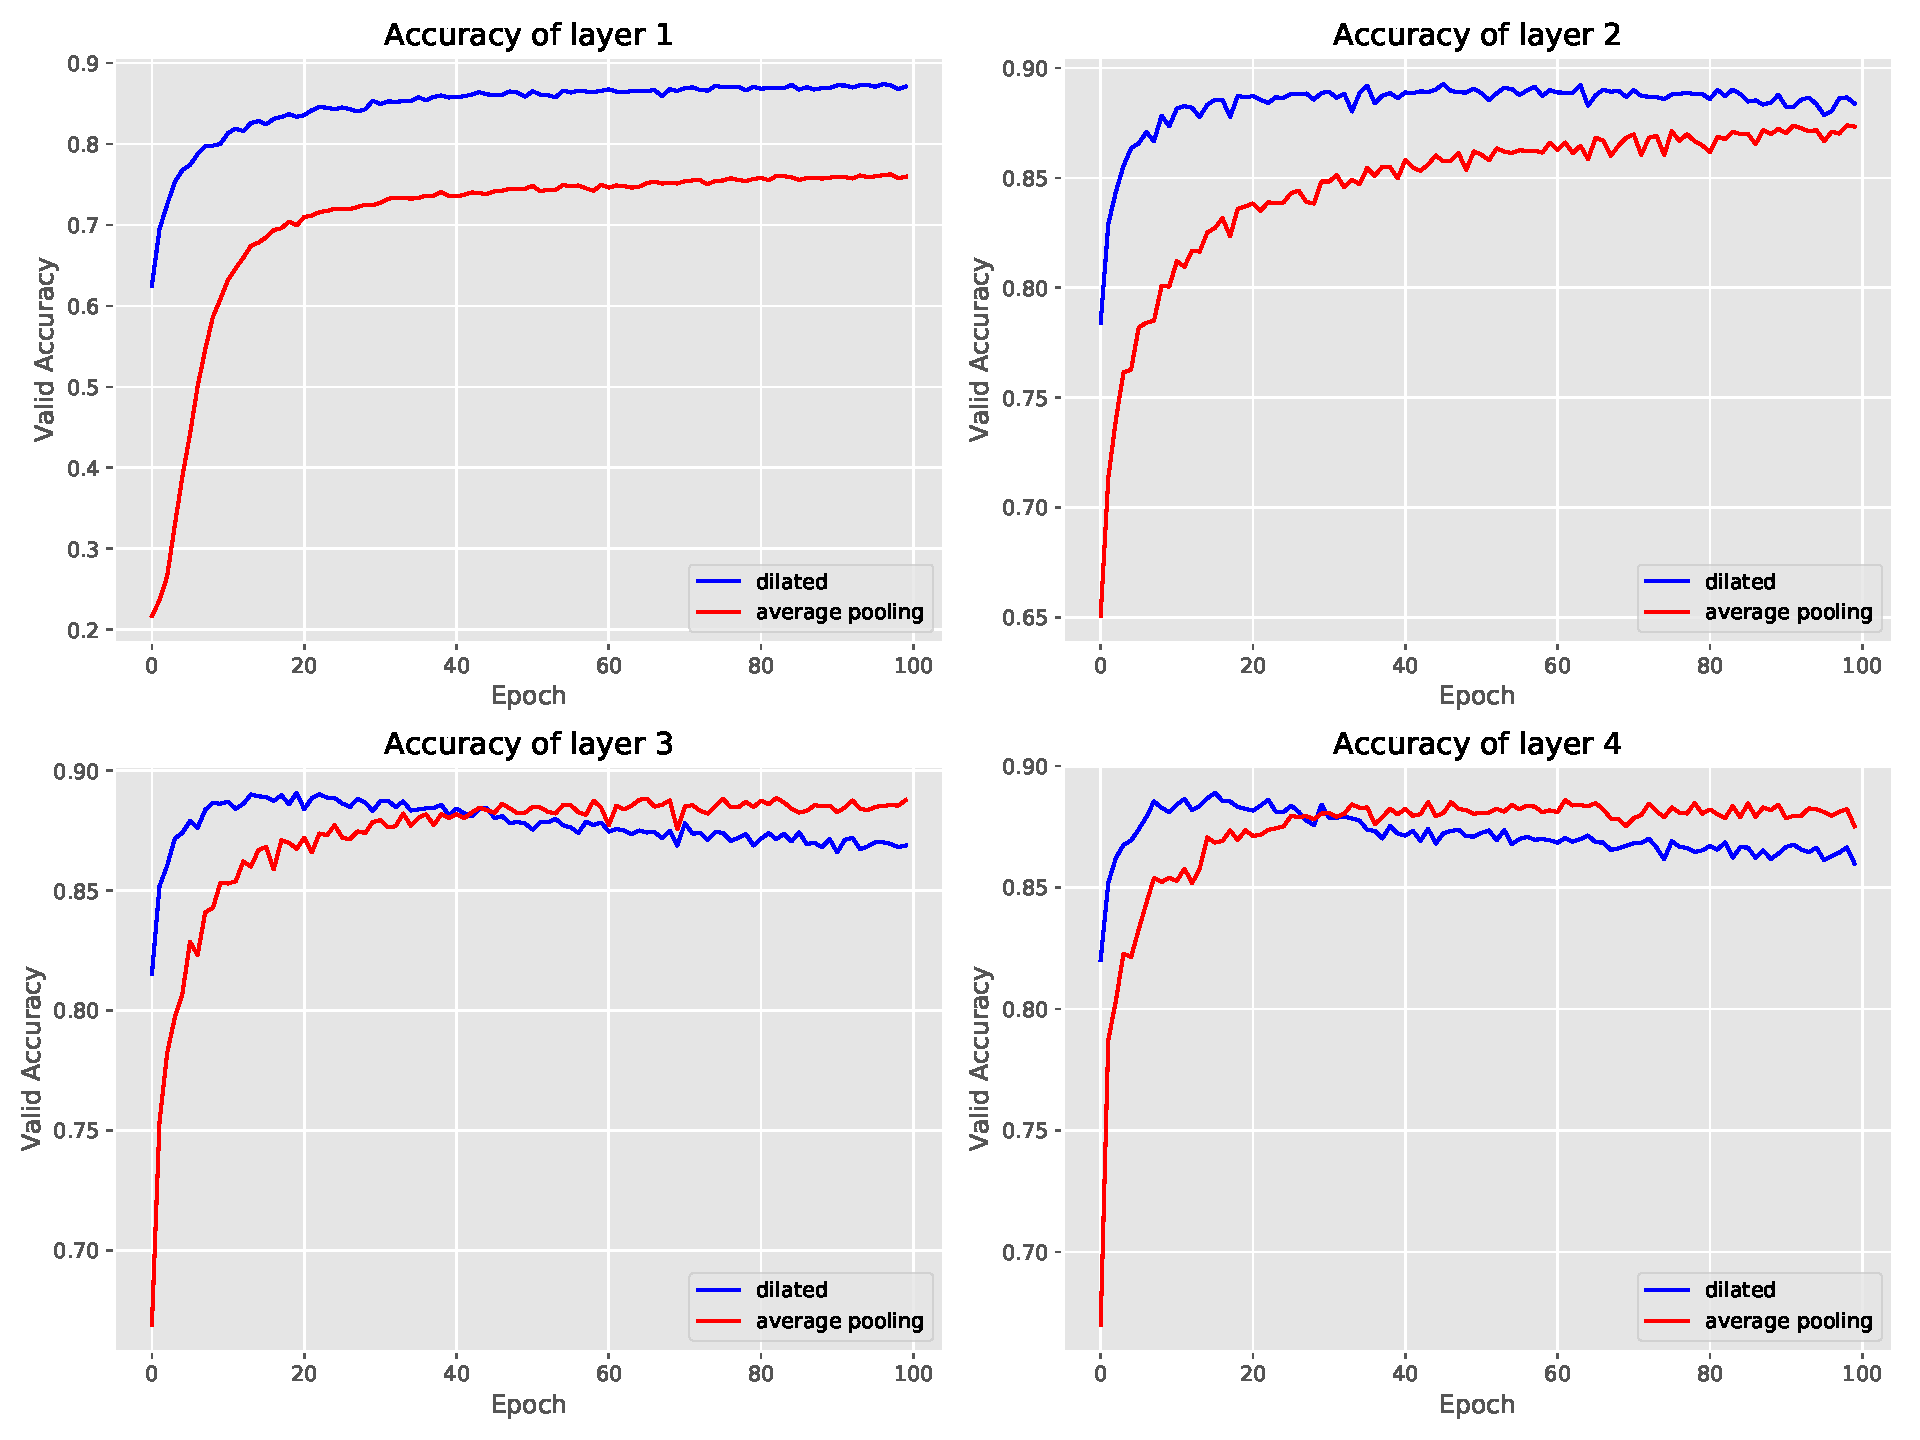
\includegraphics[width=0.44\textwidth]{./pic/part2/dilated_average_layer_acc.pdf} %插入图片,[]中设置图片大小,{}中是图片文件名
	\caption{Accuracy of different layers with filter = 32} %最终文档中希望显示的图片标题
	\label{Fig.main2} %用于文内引用的标签
\end{figure}

\begin{figure}[H] %H为当前位置,!htb为忽略美学标准,htbp为浮动图形
	\centering %图片居中
	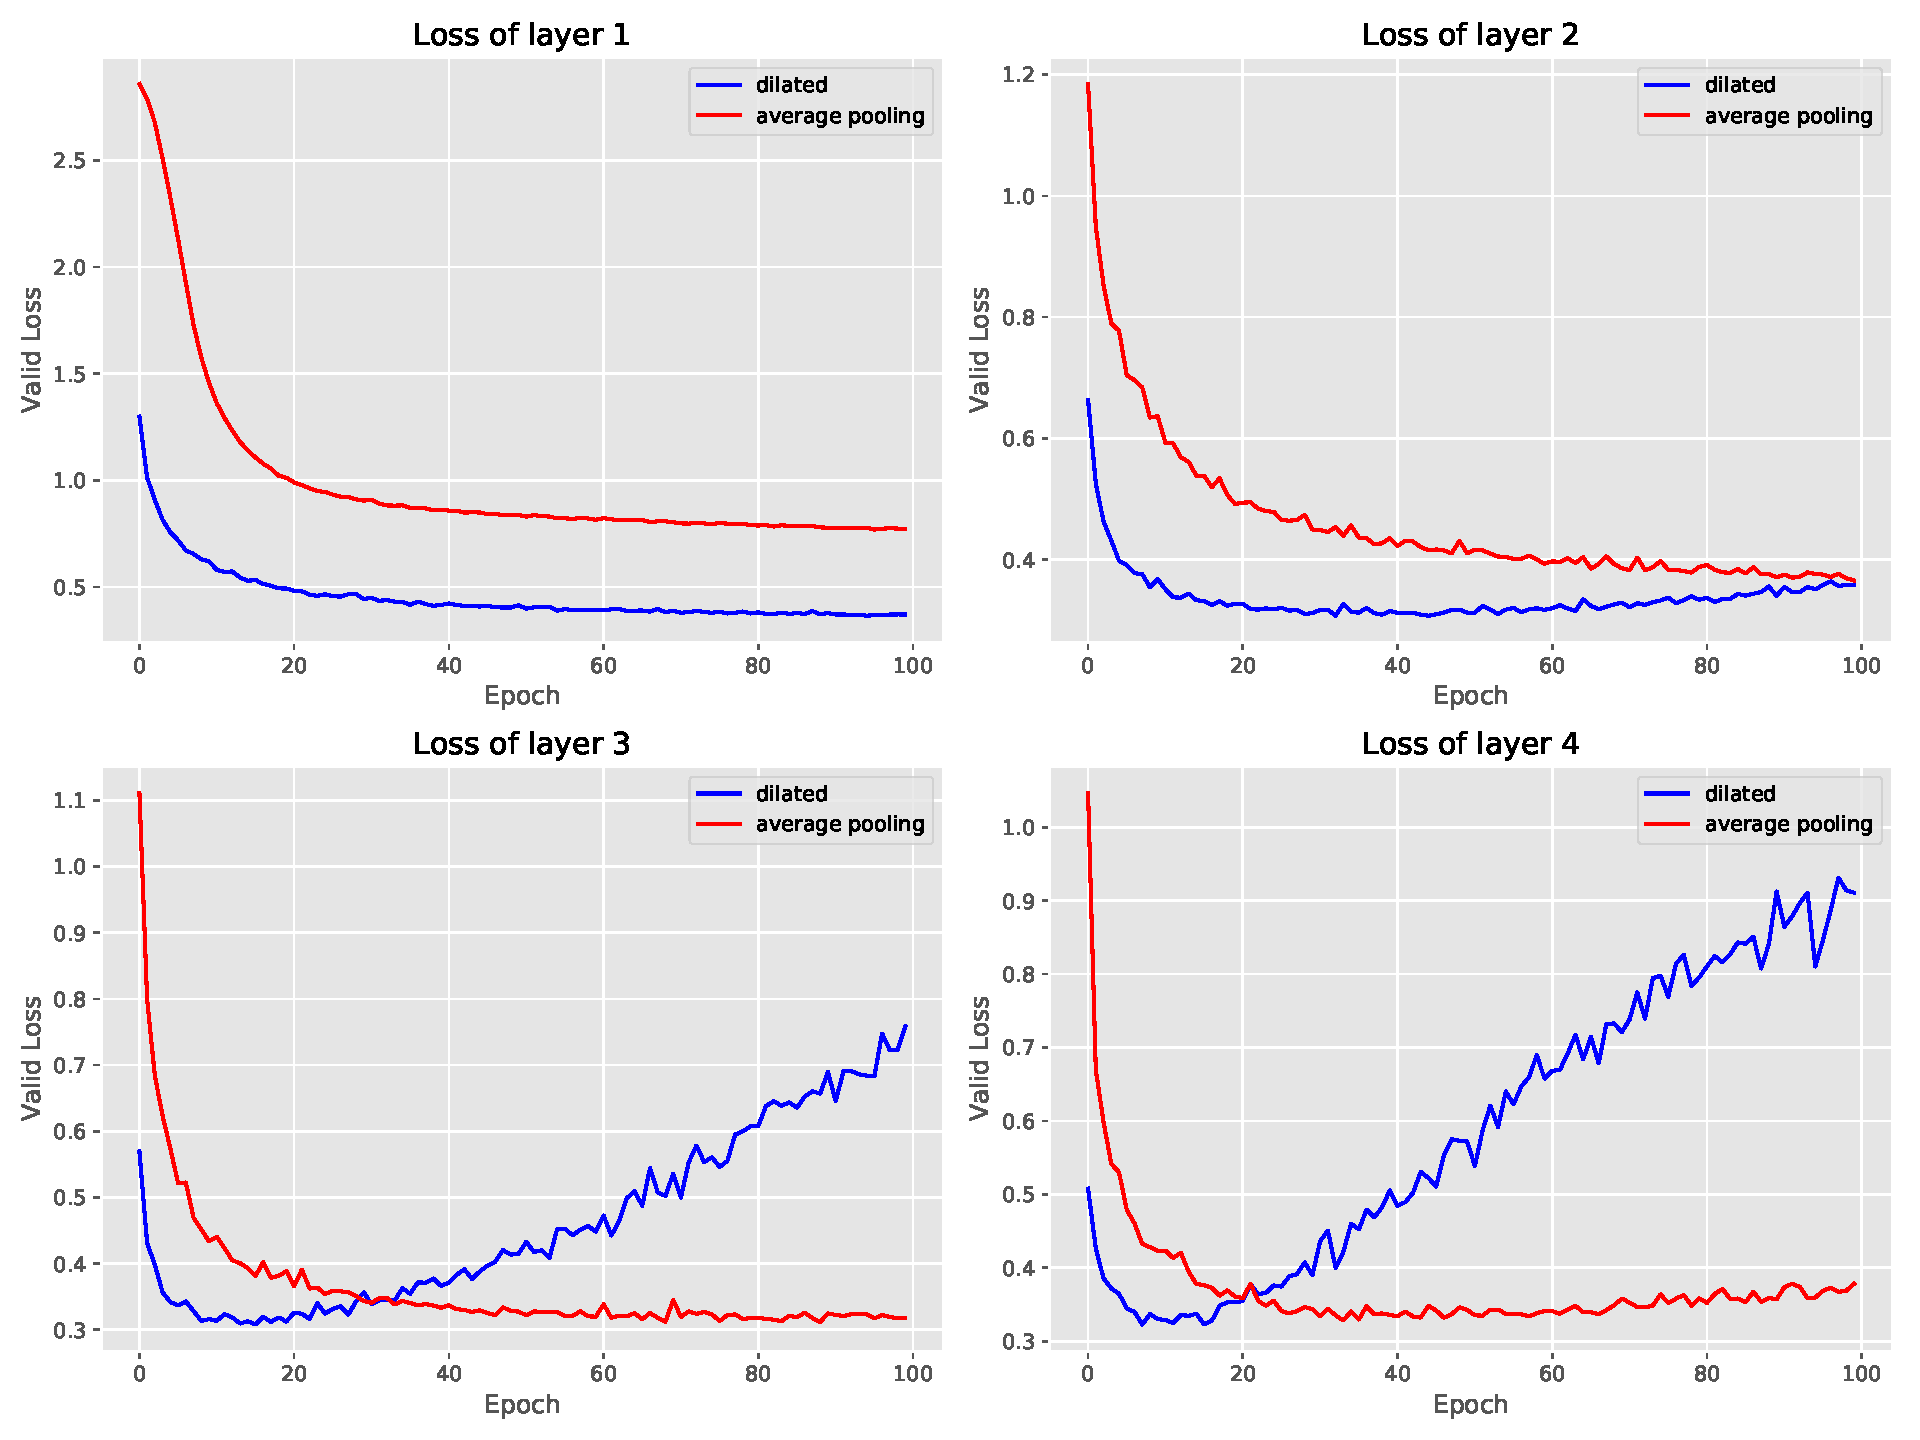
\includegraphics[width=0.44\textwidth]{./pic/part2/dilated_average_layer_loss.pdf} %插入图片,[]中设置图片大小,{}中是图片文件名
	\caption{Loss of different layers with filter = 32} %最终文档中希望显示的图片标题
	\label{Fig.main2} %用于文内引用的标签
\end{figure}

In this experiment I will change the layer from 1 to 4 and use the hyperparameter filter=32. Because when filter=64, the extracted features are too many, it is easy to produce over-fitting when layer=4.

\textbf{Accuracy}

% Table generated by Excel2LaTeX from sheet 'Sheet1'
\begin{table}[H]
  \centering
  \caption{Accuracy of Different layers for Test set}
    \begin{tabular}{lrr}
          & \multicolumn{1}{l}{average pooling} & \multicolumn{1}{l}{dilated convolutional} \\
    layer1 & 0.752341772 & 0.867088608 \\
    layer2 & 0.86398734 & 0.885379747 \\
    layer3 & 0.88012658 & 0.881582278 \\
    layer4 & 0.87689873 & 0.87702532 \\
    \end{tabular}%
  \label{tab:addlabel}%
\end{table}%

From the accuracy rate, the highest accuracy rate of average pooling is when the layer is 3, and the highest accuracy of the dalided convolutional is when the layer is 2, and then the accuracy is reduced due to over-fitting. The best accuracy of dilated convolutional is slightly higher than the average pooling


\textbf{Fitting speed}
As can be seen from the accuracy graph, when the layer is 1, the accuracy of the classified convolutional is as high as 0.867, and the average pooling is still in an under-fitting state, the accuracy is only 0.75, and then when the layer is 3, 4 At the time, the classified convolutional is already in a more serious over-fitting state. The average pooling has a slight overfitting only when the layer is 4.This shows that the dilated convolutional has a very strong ability to fit and learn.

\textbf{Runtime}

% Table generated by Excel2LaTeX from sheet 'Sheet1'
\begin{table}[htbp]
  \centering
  \caption{one epoch runtime of different layer with filter = 32}
    \begin{tabular}{lrr}
          & \multicolumn{1}{l}{average pooling} & \multicolumn{1}{l}{dilated convolutional} \\
    layer=1 & 11.2   & 15.5 \\
    layer=2 & 12.81 & 24.61 \\
    layer=3 & 13.26 & 30.52 \\
    layer=4 & 15.85 & 34.64 \\
    \end{tabular}%
  \label{tab:addlabel}%
\end{table}%

As can be seen from the table, the dilated convolution runs much longer than the average pooling. When the layer is 1, the difference is 4 seconds for an epoch, and when the layer is 4, the time for the dilated convolution is twice that of the average layer.

\section{Discussion}

For the algorithm selection of the convolutional layer, the traditional naive convolution algorithm does not require additional, but the direct convolution calculation is not satisfactory in speed. Especially for deeper networks, larger pictures. Faced with massive parameters and a large number of convolution operations, the simple algorithm can not cope with it.On the contrary, although im2col requires more memory space, the speed increase is also very obvious. In the real world, we can increase the memory space relatively easily, but it is very difficult to increase the calculation speed, so it is acceptable to sacrifice space for cooking time. So most of the deep learning frameworks use this convolution algorithm now, which also verifies the validity and generality of this algorithm from the side.
The biggest reason why the Fourier algorithm can't be mainstream is that it needs to convert the kernel to the same size as input. In reality, in order to reduce the parameters and speed up the calculation, the size of the kernel is much smaller than the input. This causes the kernel to require more memory space during the conversion process, and the conversion efficiency is also low. However, if the size of the kernel is not very small, the Fourier algorithm is much more efficient than the traditional simple convolution algorithm\cite{deeplearning2016}.\\
In this experiment, the best accuracy of average pooling (0.88) is higher than max pooling (0.874). The overall accuracy rate is also higher than the max pooling. The reason I think is this: when extracting information, when pooling, if you take the mean-pooling, you can always retain the characteristics of the overall data, and can highlight the background information, and if you take the maximum value of the region ( Max-pooling), it is better to retain the features on the texture. Because the images of EMNIST are all black and white, the background features are better, and max pooling may lose some features when selecting the largest feature. In the real world, we are faced with colored images. The way max pooling selects texture features makes it easier to find important features of the image.In terms of fitting speed, because max pooling selects the region maximum, and average pooling selects the region average. The max pooling method is more direct and easier to select the largest feature, so max pooling fits much faster than average.\\
This is a discussion about average pooling and dilated convolution. Both are methods of downsampling. The downsampling method is mainly to reduce the parameters. For the receptive field, the average pooling does not change, and the dilated convolution can expand the receptive field with the increase of the level. The big receptive field allows the network to learn more features, so you can see that the accuracy of the classified convolution (0.885) is better than the average pooling (0.880). Receptive field expansion, learning more features, can also speed up the fitting speed. However, this also brings some problems. When the receptive field expands, more features are learned. This may bring about an over-fitting problem. And the expansion of the receptive field will increase the amount of calculation, so we see that each dilated convolution runs much slower than the average pooling.






\section{Conclusions}
\label{sec:concl}
In conclusion,because most of the computational time of convolutional neural networks is spent in the convolutional layer, the im2col method sacrifices space for more computational speed, which is acceptable.Max pooling has a faster fitting speed than average pooling, but the accuracy is slightly lower than average pooling. Dilated convolution has higher accuracy and faster fitting speed than pooling fuction, but it can not neglect the over-fitting problem and the long-running problem.


\bibliography{example-refs}

\end{document} 

